\documentclass[10pt,a4paper]{article}
\usepackage[latin1]{inputenc}
\usepackage{amsmath}
\usepackage{amsfonts}
\usepackage{amssymb}
\usepackage{graphicx}
\author{Raul Persa, Lukas Vogel}
\title{Exercise 3 - Functional Specification}
\begin{document}
	\maketitle
	
\section{Objectives}

\subsection{Mandatory criteria}
	\begin{itemize}
		\item \textbf{Analysis}
			\begin{itemize}
				\item Composition of the Bundestag by party, taking into consideration: Direkt-, \"Uberhangs- and Ausgleichsmandate. Figure~\ref{fig:hp}.
			
				\item Overview for each Wahlkreis. Figure~\ref{fig:wkreis}.
			
				\item Each vote has to be stored separately.
			
				\item Compare results of current elections to former elections, especially those from 2009 and 2013
			\end{itemize}

		\item \textbf{Voting}
			\begin{itemize}
				\item Accept and store votes from people who are eligible to vote.
				
				\item Only one first and second vote per person allowed				
			\end{itemize}
		
		\item \textbf{Privacy}
			\begin{itemize}
				\item Votes have to be completely anonymous.
				\item Access to sensitive information (voters, adresses, names, \dots) is to be restricted in such a way as to guarantee privacy.
				\item Reports are only generated when data sizes are large enough to guarantee anonymity.
			\end{itemize}
			
		\item \textbf{Robustness}
			\begin{itemize}
				\item Consistent state even after power loss or resetting of the system.
			\end{itemize}
			

		\item \textbf{Scalability}
			\begin{itemize}
				\item An input of 150 million votes can be handled in 12 hours.
				\item Over the next 6 hours after voting has ended: 200,000 requests per minute can be handled at peak. 
			\end{itemize} 
			
		\item \textbf{Performance}
			\begin{itemize}
				\item The average vote has to be registered in less than 15 seconds.
				\item Calculation of the partial election results in less than 10 minutes.
				\item A web-page, showing the current election status has to be served in less than 20 seconds.
			\end{itemize}
			
		\item \textbf{Security}: The system has to be SQL-Injection-proof.
	\end{itemize}
\subsection{Desired criteria}
	\begin{itemize}
		\item \textbf{Security}: The system has to reasonably resist attempts of intrusion or disruption (e.g. DDoS \dots)
		
		\item \textbf{Performance}
			\begin{itemize}
				\item The vote has to be registered in less than 5 seconds.
				\item A web-page, showing the current election status has to be served in less than 2 seconds on average.
			\end{itemize}
	\end{itemize}
\subsection{Optional critria}
	\begin{itemize}
		\item Votes can be aggregated on Wahlkreis-level for faster analysis.
		\item Votes from former elections don't have to be kept.
	\end{itemize}

\subsection{Demarcation criteria}
	\begin{itemize}
		\item No full compliance with the BWahlGV (partial results during running election, \dots).
		\item Voting Frontend running not only on hardware compliant with the BWahlGV.
	\end{itemize}
	
	
\section{Technical implementation}
	\begin{itemize}
		\item \textbf{DBMS} storing the data specified in the data model.
		\item \textbf{Application Server} allows access to the data while ensuring privacy and security.
		\item \textbf{Web-Frontend} to show an analysis of the gathered data.
		\item \textbf{Voting-Terminal} has access to the database over the Application Server to register votes.
	\end{itemize}

\section{GUI-Mockups}
See figures~\ref{fig:hp} to \ref{fig:voting}.

\section{Data Model}
See Figure~\ref{fig:model}.

\newpage


\begin{figure}
	\centering
	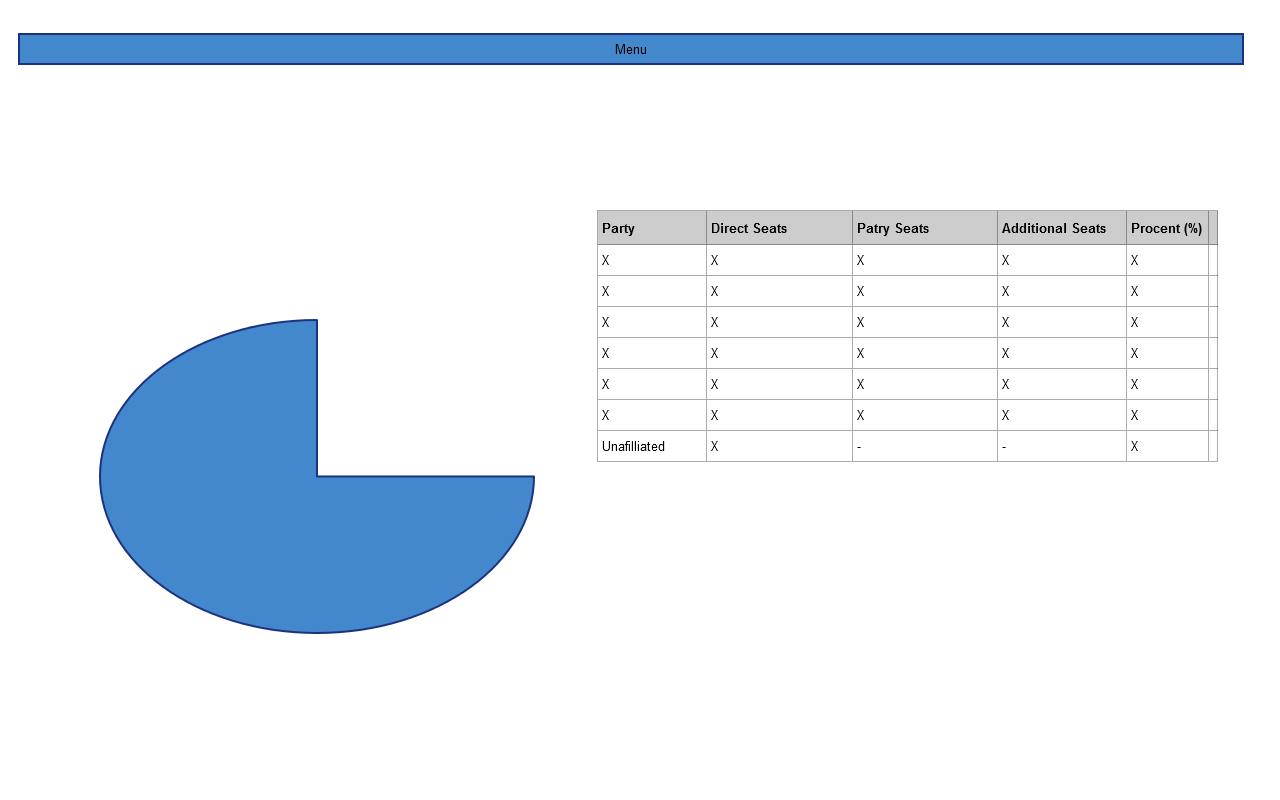
\includegraphics[scale=.3]{HomePage.png}
	\caption{Homepage}
	\label{fig:hp}
\end{figure}

\begin{figure}
	\centering
	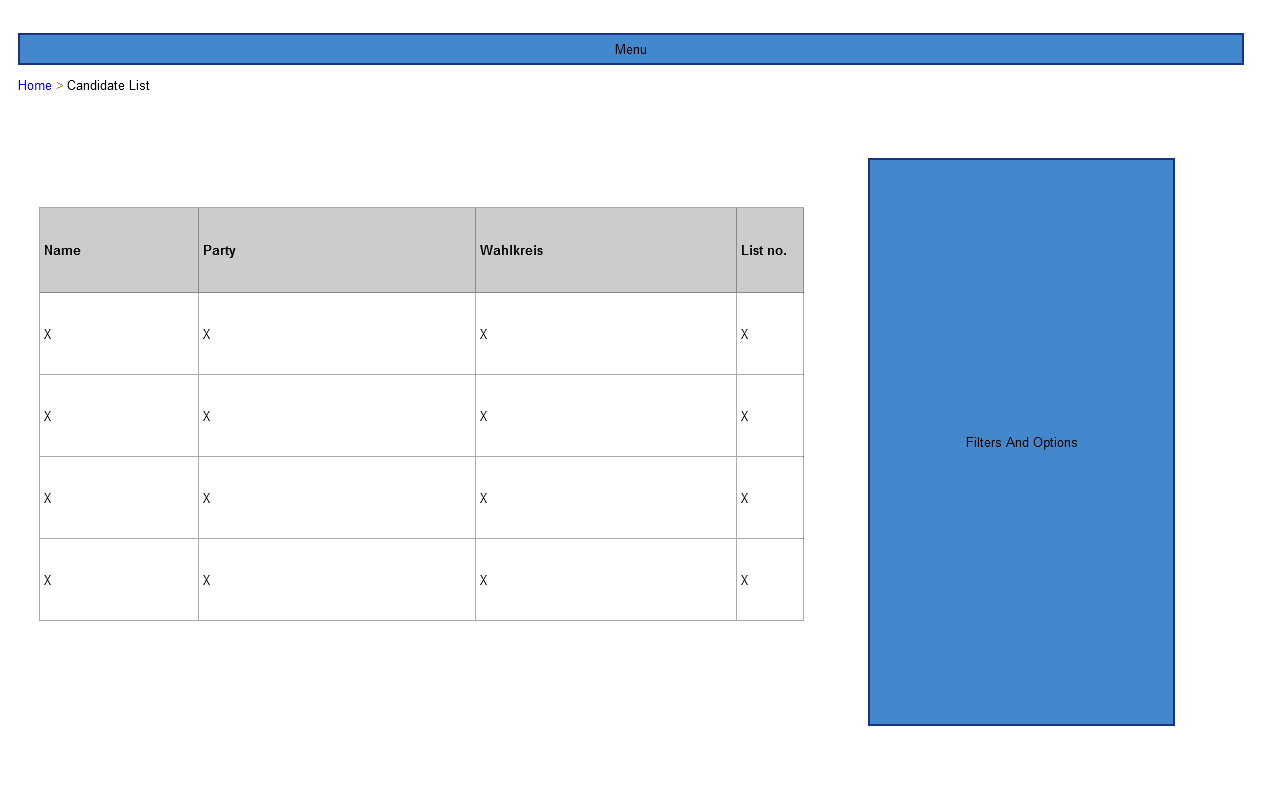
\includegraphics[scale=.3]{CandidateList.png}
	\caption{Candidate List}
	\label{fig:clist}
\end{figure}



\begin{figure}
	\centering
	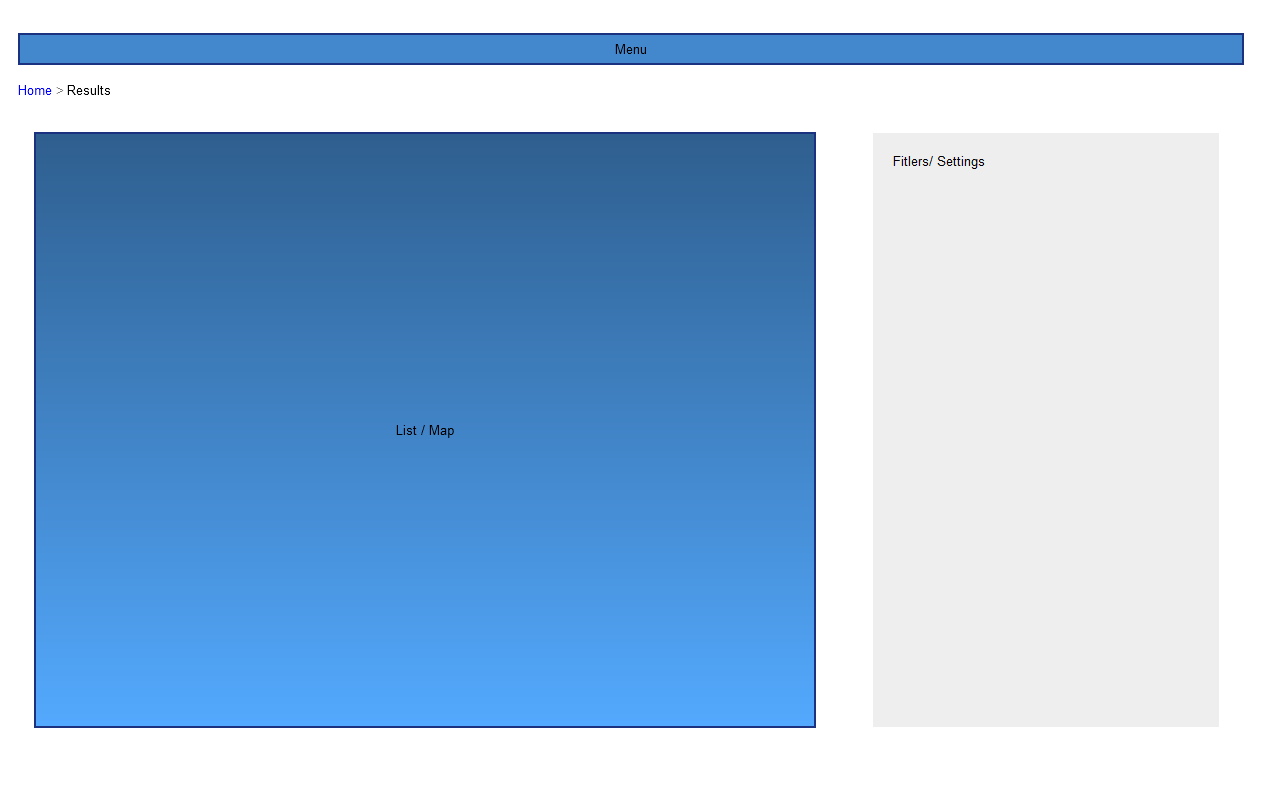
\includegraphics[scale=.3]{Results.png}
	\caption{Overview Wahlkreise}
	\label{fig:results}
\end{figure}

\begin{figure}
	\centering
	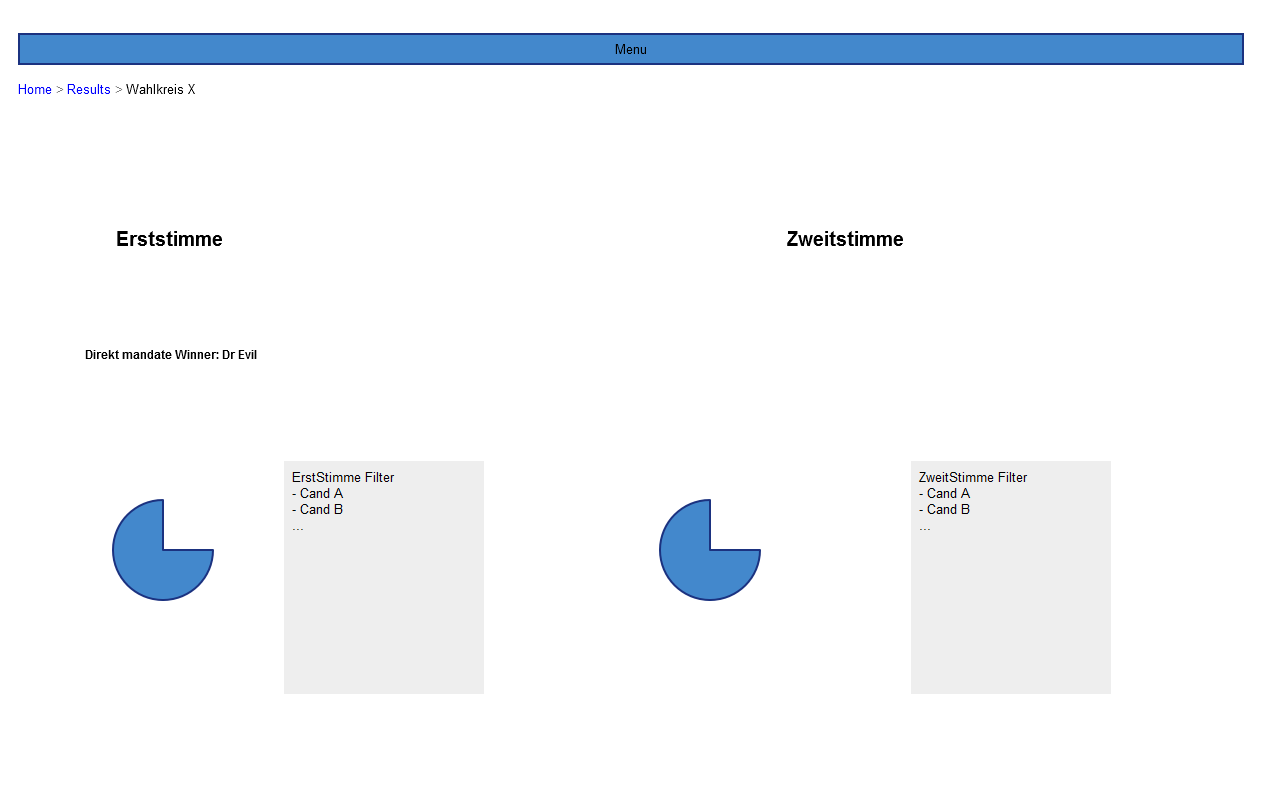
\includegraphics[scale=.3]{Wahlkreis.png}
	\caption{Detailed view for Wahlkreis}
	\label{fig:wkreis}
\end{figure}

\begin{figure}
	\centering
	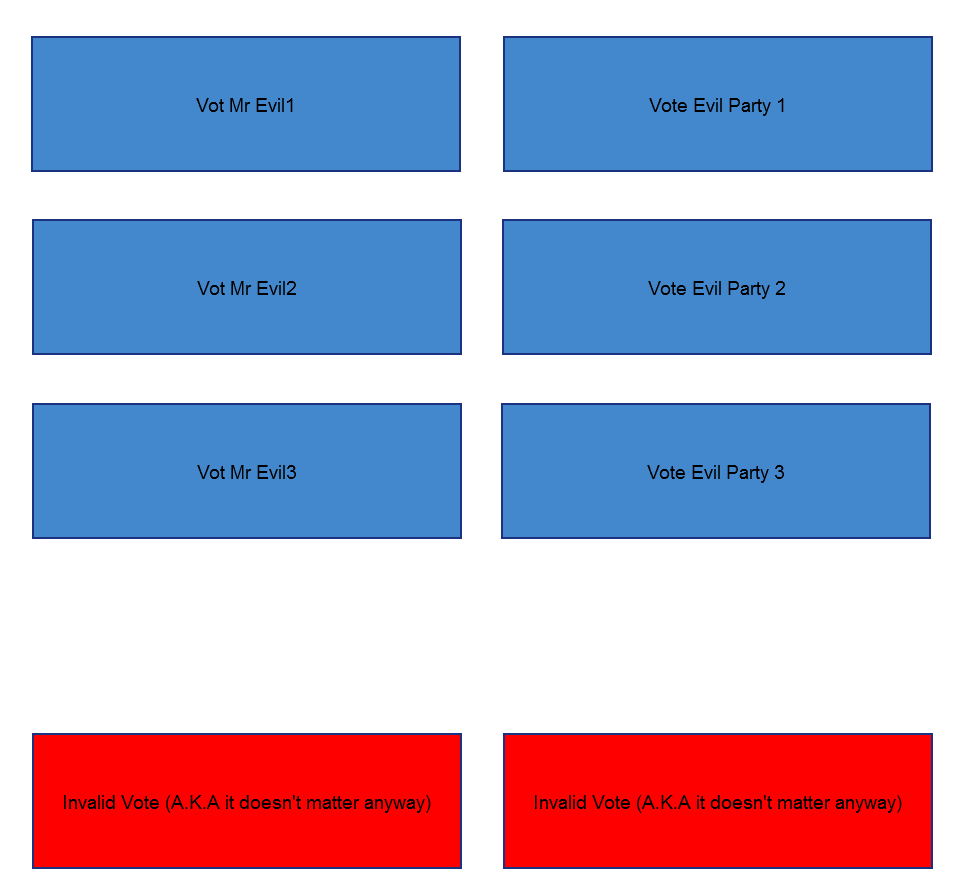
\includegraphics[scale=.3]{VotingGUI.png}
	\caption{Voting GUI}
	\label{fig:voting}
\end{figure}



\begin{figure}
	\centering
	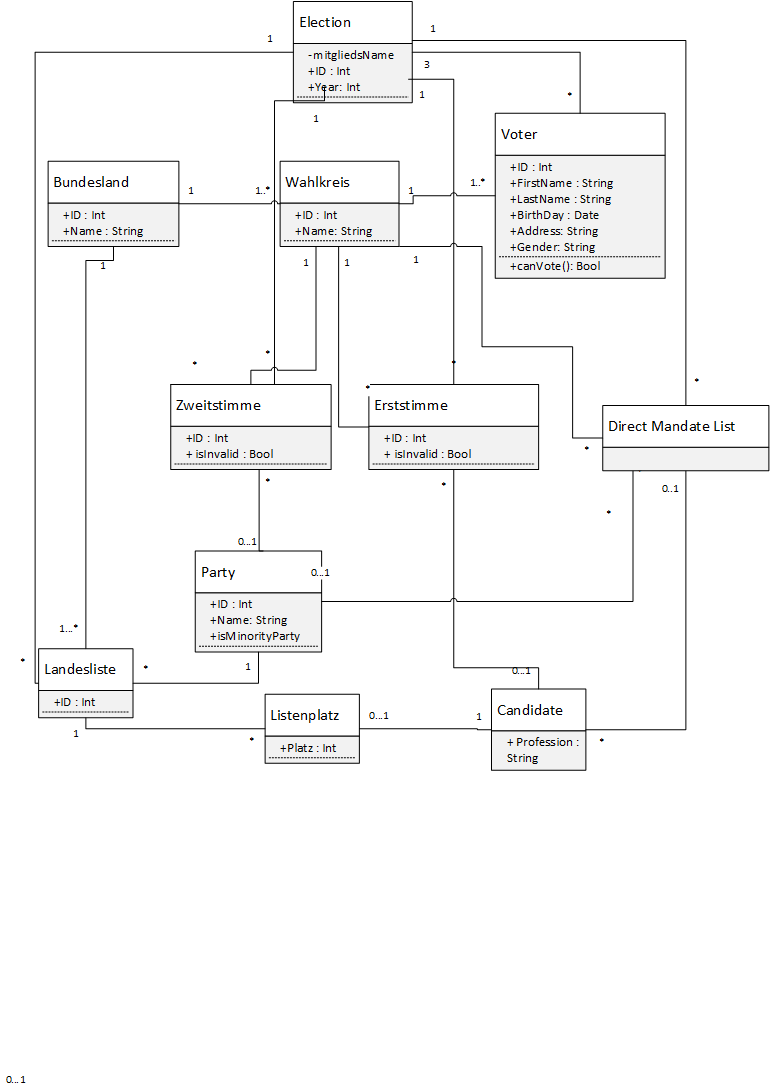
\includegraphics[scale=.8]{../Wahlschema.png}
	\caption{Data Model}
	\label{fig:model}
\end{figure}




\end{document}